\documentclass[11pt,letterpaper]{article}

% ===================== PACKAGES =====================
\usepackage[utf8]{inputenc}
\usepackage[english]{babel}
\usepackage[T1]{fontenc}
\usepackage[margin=2.5cm]{geometry}
\usepackage{amsmath,amssymb}
\usepackage{graphicx}
\usepackage{booktabs}
\usepackage{array}
\usepackage{makecell}
\usepackage{xcolor}
\usepackage{siunitx}
\usepackage{hyperref}
\usepackage{enumitem}
\usepackage{caption}
\usepackage{fancyhdr}
\usepackage{tcolorbox}
\usepackage{float}
\tcbuselibrary{skins,breakable}

\hypersetup{
    colorlinks=true,
    linkcolor=blue!50!black,
    citecolor=blue!50!black,
    urlcolor=blue!50!black
}

\sisetup{output-decimal-marker={.}, group-separator={,}}

\setlength{\headheight}{14pt}
\pagestyle{fancy}
\fancyhf{}
\fancyhead[L]{Hot-Swap eFuse (LTC4215) -- Project Logbook}
\fancyhead[R]{\thepage}
\renewcommand{\headrulewidth}{0.4pt}

\newtcolorbox{pending}{colback=yellow!8,colframe=orange!60!black,arc=1mm,breakable,title={PENDING}}

% ===================== DOCUMENT METADATA =====================
\title{\textbf{A 12\,V Hot-Swap / eFuse Front-End Using the LTC4215} \\[4pt]
\large Electronic Engineering Technical Documentation}
\author{Project Logbook}
\date{Version 0.1 --- \today}

\begin{document}

\maketitle

\begin{abstract}
\noindent This document describes the design, LTspice validation, and KiCad schematic/PCB layout of a
12\,V hot-swap / eFuse front-end built around the LTC4215 hot-swap controller. It is a deliberately small
project in the same series as the LM317, LM2596, and LTC1929 VRM projects -- chosen specifically to add a
fast, self-contained result to the portfolio without derailing the in-progress 2-phase VRM work, while
still being directly on-theme for a server/GPU power-delivery specialization (live board insertion, inrush
limiting, and electronic circuit breaking are the Phase~3 ``server-specific power topics'' item on that
roadmap). Documented as an honest engineering logbook: every result is marked as \textbf{calculated},
\textbf{simulated}, or \textbf{pending} -- never filled in with invented placeholder data. \textbf{Key
result}: the controlled startup, the automatic recovery from an undervoltage (UV) event, and the permanent
latch-off on a hard output short were all reproduced and numerically verified from the LTspice
\texttt{.raw} file (not read visually from plots), matching the design's calculated circuit-breaker
threshold (\SI{5}{\ampere}) and confirming the LTC4215's documented UV auto-retry and OC latch-off
behavior. The KiCad schematic and 2-layer PCB layout are complete, ERC/DRC clean, and not yet
sent to fabrication (simulation + layout only, confirmed project scope).
\end{abstract}

\tableofcontents
\newpage

% ======================================================================
\section{Project Objective}

Design and validate, in LTspice, a 12\,V hot-swap / electronic-fuse (eFuse) front-end using a real hot-swap
controller IC (LTC4215): a MOSFET series pass switch whose gate is ramped under closed-loop control at
insertion, with input undervoltage/overvoltage lockout and a fast, non-resettable circuit-breaker response
to a downstream short. Scope agreed for this project: LTspice simulation first (this document), KiCad
schematic/PCB afterward -- not a build.

% ======================================================================
\section{Controller Selection}

\subsection{Why hot-swap/eFuse, and why now}

This project reaches ahead to the ``server-specific power topics'' item of the longer-term roadmap (hot-
swap/eFuse, power sequencing, digital power/PMBus) rather than following the roadmap strictly in order,
deliberately chosen as a small, fast, self-contained result while the 2-phase VRM (\texttt{VRM\_2PHASE\_
LTC1929}) layout is in progress. It stays on-theme for the stated specialization (server/GPU board power
delivery) instead of diluting the portfolio with an unrelated topic.

\subsection{IC selection: LTC4215}

Confirmed present in the local LTspice installation: SPICE subcircuit model (\texttt{LTC4215.sub}) and
schematic symbol (\texttt{PowerProducts/LTC4215.asy}), both verified directly against the real datasheet
pinout before use -- not assumed. LTC4215 is a hot-swap controller with an external N-channel pass
MOSFET, adjustable foldback current limiting, a programmable soft-start (dI/dt) ramp, input UV/OV lockout,
and an independent, fast circuit-breaker comparator -- a real part used in ``Computers, Servers'' and
``Platform Management'' applications per its own datasheet.

\subsection{Package decision: QFN-24 vs.\ SSOP-16}

The datasheet's simplified pinout comparison revealed a real functional difference between packages, not
just a footprint choice:

\begin{center}
\begin{tabular}{@{}lll@{}}
\toprule
& \textbf{SSOP-16 (GN)} & \textbf{QFN-24 (UFD)} \\
\midrule
OV pin & absent & present \\
$\overline{\text{EN}}$ pin & absent & present \\
SENSE$^+$ & tied internally to V$_{DD}$ & separate external pin \\
ADIN, ADR1, ADR2 & absent & present \\
\bottomrule
\end{tabular}
\end{center}

This design uses the OV protection pin, so the \textbf{QFN-24 package is required} (the SSOP-16 cannot
implement the OV divider at all). The LTspice macromodel exposes the full pin set regardless of package,
so the simulation is package-agnostic.

\textbf{Resolved (Section~\ref{sec:pcb}):} symbol/footprint/3D model for \texttt{LTC4215IUFD-1\#PBF}
(SnapEDA, via DigiKey) -- a real, in-production part confirmed against its own datasheet
(\texttt{421513fc.pdf}, Rev.\ C) to be electrically equivalent to the LTC4215 modeled in Section~2.2 for
every feature this project uses.

% ======================================================================
\section{Datasheet Review}

Transcribed directly from the LTC4215/LTC4215-2 datasheet (Linear Technology/Analog Devices, Rev.\ E),
\texttt{docs/LTC4215\_Datasheet.pdf}.

\begin{table}[H]
\centering
\small
\caption{LTC4215 key parameters}
\begin{tabular}{@{}p{7cm}p{4cm}p{1cm}@{}}
\toprule
\textbf{Parameter} & \textbf{Value} & \textbf{p.} \\
\midrule
Supply voltage range, $V_{DD}$ & \SI{2.9}{}--\SI{15}{\volt} & 3 \\
$V_{DD}$ undervoltage lockout (rising) & \SI{2.84}{\volt} typ & 3 \\
$V_{DD}$ overvoltage lockout & \SI{15.6}{\volt} typ & 3 \\
UV/OV/ON/FB comparator threshold & \SI{1.235}{\volt} typ (all four) & 4 \\
Circuit breaker threshold, $\Delta V_{SENSE(TH)}$ & \SI{25}{\milli\volt} typ & 3 \\
OC fault filter, $t_{D(OC)}$ (LTC4215) & \SI{20}{\micro\second} typ & 3 \\
Steady-state current limit, $\Delta V_{SENSE}$ (post-startup) & \SI{75}{\milli\volt} typ & 3 \\
External gate drive, $\Delta V_{GATE}$ & \SI{5.9}{\volt} typ (4.7--6.5) & 3 \\
Package & 16-lead SSOP or 24-pin QFN & 2 \\
\bottomrule
\end{tabular}
\end{table}

\textbf{SS pin:} sets the inrush dI/dt. Datasheet's own calibration point: \SI{68}{\nano\farad} on SS
gives a \SI{5}{\milli\volt\per\milli\second} sense-voltage ramp (p.9), i.e.\ \SI{1}{\ampere\per
\milli\second} with $R_{SENSE}=\SI{5}{\milli\ohm}$.

\textbf{TIMER pin:} normally a capacitor sets a \SI{12.3}{\milli\second\per\micro\farad} start-up watchdog
duration. \textbf{Documented alternate mode, used here}: ``An internal timer provides a \SI{100}{\milli
\second} start-up time and \SI{5}{\second} auto-retry time if this pin is tied to INTV$_{CC}$'' (p.9) --
simpler than computing a custom RC value, and \SI{100}{\milli\second} is ample margin over this design's
calculated charge time (Section~\ref{sec:results}).

\textbf{ON pin:} ``if the ON pin is tied high, then the FET On bit goes high \SI{100}{\milli\second} after
power-up'' (p.8) -- the same \SI{100}{\milli\second} delay as above, and critical to the simulation
debugging in Section~\ref{sec:pitfalls}.

% ======================================================================
\section{Design}
\label{sec:design}

\subsection{Design targets}

\begin{center}
\begin{tabular}{@{}ll@{}}
\toprule
$V_{DD}$ & \SI{12}{\volt} (project-wide rail) \\
Circuit breaker trip & \SI{5}{\ampere} (fast, non-resettable: $ocautoretry=0$) \\
Steady-state current limit & \SI{15}{\ampere} (post-startup foldback release) \\
\bottomrule
\end{tabular}
\end{center}

\subsection{Reference design: adapted from Datasheet Figure 1}

Figure 1 (``12V Application with 5A Circuit Breaker'') was adopted as the base reference -- a real,
manufacturer-validated 12\,V application circuit, directly matching this project's target rail and current
class. \textbf{System-level simplification:} Figure 1 shows two mating connectors (Connector 2 =
backplane socket, Connector 1 = plug-in card edge, carrying both the power pins and the I$^2$C signaling
pins to a backplane management controller). Without a backplane chassis to build, this project collapses
both to a single input connector carrying only the 12\,V/GND power pair; the I$^2$C signaling pins (SDA,
SCL, $\overline{\text{ALERT}}$, ADR0--2, ADIN, GPIO) are left unused (Section~\ref{sec:scope}).

\subsubsection{I$^2$C scope decision}
\label{sec:scope}

This project uses only the LTC4215's analog hot-swap functionality (soft-start, UV/OV, current limit,
circuit breaker) -- no I$^2$C monitoring. Two independent reasons: (1) keeping the project small and
self-contained, matching its role as a fast portfolio addition; (2) the local LTspice macromodel does not
even expose SDA/SCL/$\overline{\text{ALERT}}$/ADR0--2/ADIN as separate pins (confirmed from the \texttt{
.asy} pin list), so I$^2$C could not be simulated here regardless.

\begin{pending}
A follow-on project (already on the longer-term roadmap, Phase 3) is to add an STM32 minimal system
reading the LTC4215's I$^2$C telemetry (8-bit ADC monitoring current/voltage) -- the natural bridge between
this project's power-electronics work and embedded-systems work. Not started.
\end{pending}

\subsubsection{Component values}

\begin{center}
\begin{tabular}{@{}lll@{}}
\toprule
\textbf{Component} & \textbf{Value} & \textbf{Source / derivation} \\
\midrule
$R_{SENSE}$ (R6) & \SI{5}{\milli\ohm} & matches datasheet's own SS calibration point \\
$M_1$ & Si7336ADP & see Section~\ref{sec:mosfet} \\
$D_1$ (TVS, real BOM) & P6KE16A & Fig.~1 (surge suppressor, $V_{DD}$--GND) \\
$D_1$ (SPICE substitute) & BZX84C15L & see Section~\ref{sec:tvs} \\
$R_5$/$R_4$/$R_3$ (UV/OV string) & \SI{34.8}{\kilo\ohm} / \SI{1.18}{\kilo\ohm} / \SI{3.4}{\kilo\ohm} & Fig.~1, verified by calculation below \\
$C_3$ & \SI{0.1}{\micro\farad} & Fig.~5 (noise bypass at UV/OV node) \\
$R_7$/$R_8$ (FB divider) & \SI{30.1}{\kilo\ohm} / \SI{3.57}{\kilo\ohm} & Fig.~1 \\
$C_1$ (SS) & \SI{68}{\nano\farad} & Fig.~1; sets \SI{1}{\ampere\per\milli\second} inrush ramp \\
TIMER & tied to INTV$_{CC}$ & datasheet alternate mode (Section~3) \\
ON & tied to INTV$_{CC}$ & auto-start at power-up \\
$\overline{\text{EN}}$ & tied to GND & board always present (no mechanical detect) \\
$R_1$ (gate) & \SI{10}{\ohm} & series gate-drive damping \\
$R_2$ (GPIO pull-up) & \SI{24}{\kilo\ohm} to INTV$_{CC}$ & Fig.~1; power-good flag, kept even without I$^2$C \\
$C_4$ ($C_L$, output) & \SI{12}{\milli\farad} & datasheet's own Start-Up Waveform test condition \\
\bottomrule
\end{tabular}
\end{center}

\textbf{UV/OV string, verified by calculation.} A single resistor string from $V_{DD}$ to GND
($R_5=\SI{34.8}{\kilo\ohm}$, $R_4=\SI{1.18}{\kilo\ohm}$, $R_3=\SI{3.4}{\kilo\ohm}$) feeds both comparators:
the UV tap sits between $R_5$ and $R_4$, the OV tap between $R_4$ and $R_3$. Total
$R_5+R_4+R_3=\SI{39.38}{\kilo\ohm}$. With both comparator thresholds at \SI{1.235}{\volt}:

\begin{equation}
V_{DD,\,UV\,trip} = 1.235 \times \frac{39.38}{R_4+R_3} = 1.235\times\frac{39.38}{4.58} = \boxed{\SI{10.62}{\volt}} \text{ (falling)}
\end{equation}
\begin{equation}
V_{DD,\,OV\,trip} = 1.235 \times \frac{39.38}{R_3} = 1.235\times\frac{39.38}{3.4} = \boxed{\SI{14.30}{\volt}} \text{ (rising)}
\end{equation}

\noindent i.e.\ roughly $-12\%$/$+19\%$ around the \SI{12}{\volt} nominal rail -- sensible UV/OV margins,
confirming the transcribed resistor values are self-consistent and not misread.

\textbf{FB (power-good) divider, verified similarly:} $R_7=\SI{30.1}{\kilo\ohm}$,
$R_8=\SI{3.57}{\kilo\ohm}$, total \SI{33.67}{\kilo\ohm}:

\begin{equation}
V_{OUT,\,power\,bad} = 1.235\times\frac{33.67}{3.57} = \boxed{\SI{11.65}{\volt}}
\end{equation}

\noindent power-bad is flagged below $\approx97\%$ of nominal -- a typical margin.

\subsubsection{MOSFET}
\label{sec:mosfet}

Figure 1's real BOM choice (FDC653N) has no SPICE model in the local LTspice installation. Rather than
searching for a new part, this project reuses \textbf{Si7336ADP} (Vishay PowerPAK SO-8) -- already verified
with a real SPICE model and a hand-built, datasheet-checked KiCad footprint in the
\texttt{VRM\_2PHASE\_LTC1929} project. $V_{DS}=\SI{30}{\volt}$ (ample margin over the \SI{14.3}{\volt} OV
trip), $R_{ON}=\SI{2.4}{\milli\ohm}$ typ (negligible conduction loss at this design's currents),
$V_{to}=\SI{2.9}{\volt}$ (comfortably below the LTC4215's \SI{4.7}{}--\SI{6.5}{\volt} gate drive).

\textbf{Resolved:} Si7336ADP confirmed as the final BOM part (not the datasheet's original FDC653N) --
reusing a simulated-and-laid-out part beats re-validating a new one for this project's scope. See
Section~\ref{sec:pcb} for a footprint/symbol pin-mapping issue this choice ran into.

\subsubsection{TVS substitute for simulation}
\label{sec:tvs}

The real BOM part (P6KE16A, a power TVS) has no local SPICE model. \textbf{BZX84C15L} (OnSemi,
\SI{15}{\volt} zener) is used as a simulation-only stand-in for the clamp voltage -- it reproduces the
clamping I-V behavior at low test currents but is \emph{not} power-rated for a real transient-suppression
event. The real BOM still specifies P6KE16A.

% ======================================================================
\section{SPICE Simulation (LTspice)}

\subsection{Setup}

\begin{center}
\begin{tabular}{@{}ll@{}}
\toprule
Supply, $V_1$ & step/PWL (not flat DC) -- see Section~\ref{sec:pitfalls} \\
Output load & none (bare $C_L=\SI{12}{\milli\farad}$) \\
\bottomrule
\end{tabular}
\end{center}

Numbers below come from the \texttt{.raw} file (parsed with \texttt{numpy}, time as float64 + each
variable as float32 per the LTspice binary layout, not read visually from plots).

\subsection{Two debugging pitfalls, documented for reuse}
\label{sec:pitfalls}

\textbf{Pitfall 1 -- flat DC source masks the entire power-up transient.} The first simulation attempt
used $V_1=\SI{12}{\volt}$ (flat DC). LTspice computes the transient's initial state from the circuit's own
DC operating point, which for a flat supply is self-consistent at ``board already powered, gate already
decided its state'' -- with nothing left to change over time, the solver (reached via Gmin stepping; direct
Newton failed) converged on an all-zero state and the \SI{100}{\milli\second} run showed $V_{OUT}=0$ for
its entire length. \textbf{Fix:} represent the connector-insertion event explicitly with a step source,
\texttt{PULSE(0 12 0 1u 1u 1 1)}.

\textbf{Pitfall 2 -- the \SI{100}{\milli\second} internal startup delay is easy to mistake for a dead
circuit.} Even after Pitfall 1 was fixed, $V_{OUT}$ still stayed at 0\,V for the full \SI{100}{\milli
\second} run. Tracing internal nodes (UV, OV, Gate, SS, INTV$_{CC}$/TIMER) showed every comparator settling
at its expected, correctly-calculated value, and the ON pin's INTV$_{CC}$-referenced rising edge occurring
normally around $t\approx\SI{49}{\micro\second}$ -- but the gate never moved afterward. The cause was the
documented ON-tied-high behavior (Section~3): the FET-On bit does not go high until
\SI{100}{\milli\second}\emph{after power-up}, not on the ON pin's own edge. Extending the stop time to
\SI{200}{\milli\second} reproduced the full, correct startup sequence. \textbf{Lesson: with TIMER and ON
both tied to INTV$_{CC}$, any \texttt{.tran} stop time under $\approx$\SI{150}{\milli\second} will show a
circuit that looks dead but isn't.}

\subsection{Results}
\label{sec:results}

\subsubsection{Controlled startup}

\begin{center}
\begin{tabular}{@{}ll@{}}
\toprule
Gate drive begins & $t\approx\SI{100.9}{\milli\second}$ (immediately after the internal delay) \\
SS ramp starts & $t\approx\SI{105}{\milli\second}$ \\
Inrush current peak & \textbf{\SI{5.2}{\ampere}} -- matches the \SI{5}{\ampere} circuit-breaker design target \\
$V_{OUT}$ reaches \SI{12}{\volt} & $t\approx\SI{152}{\milli\second}$ \\
Charge time ($C_L=\SI{12}{\milli\farad}$) & $\approx\SI{51}{\milli\second}$ \\
\bottomrule
\end{tabular}
\end{center}

The inrush current peak landing almost exactly at the \SI{5}{\ampere} circuit-breaker threshold (rather
than well above or below it) is a direct consequence of the foldback current-limit curve converging with
the fixed circuit-breaker threshold as FB approaches its good level -- not a coincidence, and a useful
numerical cross-check that the SS/$R_{SENSE}$ combination is sized consistently with the breaker.

\subsubsection{Undervoltage (UV) fault and automatic recovery}

Test: $V_{DD}$ stepped from \SI{12}{\volt} to \SI{8}{\volt} at $t=\SI{300}{\milli\second}$ (PWL), held for
\SI{20}{\milli\second}, returned to \SI{12}{\volt} at $t=\SI{320}{\milli\second}$.

\begin{center}
\begin{tabular}{@{}ll@{}}
\toprule
$V_{OUT}$ sags to $\approx V_{DD}$ & within $\approx\SI{300}{\micro\second}$ of the UV step \\
Mechanism & $M_1$'s body diode conducting $V_{OUT}\rightarrow V_{DD}$ (not an active pull-down) \\
$V_{DD}$ recovers & $t=\SI{320}{\milli\second}$ \\
Gate re-enables & $t\approx\SI{426}{}$--\SI{432}{\milli\second} ($\approx\SI{106}{}$--\SI{112}{\milli\second} after $V_{DD}$ recovery) \\
$V_{OUT}$ back at \SI{12}{\volt} & $t\approx\SI{477}{\milli\second}$ \\
\bottomrule
\end{tabular}
\end{center}

Two findings worth separating: (1) the fast ($\approx\SI{300}{\micro\second}$) output sag during the UV
event is \emph{not} the LTC4215 actively protecting anything -- it is the unavoidable consequence of using
a single N-channel series MOSFET as a high-side switch: once the gate turns off, the intrinsic body diode
still passes current from the (higher) output back to the (lower) input. A design needing true reverse
blocking would need back-to-back MOSFETs, not a single device. (2) The recovery delay
($\approx\SI{106}{}$--\SI{112}{\milli\second}) confirms the same internal \SI{100}{\milli\second}
startup-sequencer behavior from Section~\ref{sec:pitfalls} re-arms on every restart, not just the very
first power-up -- auto-retry ($uvautoretry=1$) is fully automatic, but not instantaneous.

\subsubsection{Overcurrent (OC) fault and permanent latch-off}

Test: a voltage-controlled switch ($R_{ON}=\SI{10}{\milli\ohm}$) closed across $V_{OUT}$ at
$t=\SI{550}{\milli\second}$ (after the UV test had already fully recovered), modeling a hard downstream
short.

\begin{center}
\begin{tabular}{@{}ll@{}}
\toprule
Total fault-path resistance & $R_{SENSE}+R_{ON,sw}+R_{DS(on)}\approx\SI{17.4}{\milli\ohm}$ \\
Theoretical instantaneous peak & $V_{OUT}/R\approx\SI{12}{\volt}/\SI{17.4}{\milli\ohm}\approx\SI{690}{\ampere}$ \\
Breaker response & trips within $t_{D(OC)}=\SI{20}{\micro\second}$ (datasheet filter) \\
$V_{OUT}$ after trip & \SI{0}{\volt}, held through the rest of the run (no recovery) \\
\bottomrule
\end{tabular}
\end{center}

The very low total fault-path resistance is exactly why the \SI{20}{\micro\second} circuit-breaker filter
matters: without a fast-acting, independent breaker comparator, this near-ideal short-circuit path could
sustain hundreds of amps rather than the \SI{5}{}--\SI{15}{\ampere} the design targets. The permanent
latch ($ocautoretry=0$, no recovery for the remainder of the \SI{700}{\milli\second} run) is the intended
behavior and the clearest contrast with the UV case above: a real overcurrent fault does not get a second
chance without an external reset.

% ======================================================================
\section{PCB Layout (KiCad)}
\label{sec:pcb}

\subsection{Library sourcing}

\textbf{U1:} symbol, footprint, and STEP model for \texttt{LTC4215IUFD-1\_PBF} sourced from SnapEDA (via
DigiKey). Its own \texttt{MPN} metadata field incorrectly read \texttt{LTC4215IUFD-2\#TRPBF} (a data-entry
error on SnapEDA's part, inconsistent with every other field on the same symbol) -- cross-checked against
the part's real datasheet (\texttt{421513fc.pdf}) before trusting it; the 24 QFN-24 pin assignments were
also independently re-verified against the datasheet's own pin configuration diagram before use, not
assumed correct because the source was reputable.

\textbf{Q1:} reused the \texttt{Transistor\_FET:Si7336ADP} symbol and \texttt{Package\_SO:
PowerPAK\_SO-8\_Single} footprint, both already validated in \texttt{VRM\_2PHASE\_LTC1929}.
\textbf{Pitfall found and fixed:} the generic \texttt{Q\_NMOS\_GSD} symbol (3 pins: 1=G, 2=S, 3=D) does
\emph{not} match this footprint's real pad numbering (pads 1--3 = Source, pad 4 = Gate, pad 5 $\times$5 =
Drain) -- using the generic symbol silently routed the Drain net onto a physical Source pad and left two
pads unconnected. The dedicated \texttt{Si7336ADP} symbol (pins 1--3=S, 4=G, 5=D) matches the footprint
exactly and resolves this with no footprint editing required.

\subsection{Assembly: SMD except where physically impossible}

All-SMD assembly, since U1 (QFN-24) and Q1 (PowerPAK SO-8) are SMD-only parts regardless -- going THT for
the passives would not simplify assembly and would only grow the board. Three exceptions, each because no
SMD option exists at the required value/rating:

\begin{center}
\begin{tabular}{@{}lll@{}}
\toprule
\textbf{Part} & \textbf{Footprint} & \textbf{Why THT} \\
\midrule
$D_1$ (P6KE16A) & \texttt{Diode\_THT:D\_DO-15\_P10.16mm\_Horizontal} & no SMD option at 600\,W peak pulse power \\
$C_4$ (\SI{12}{\milli\farad}) & \texttt{Capacitor\_THT:CP\_Radial\_D16.0mm\_P7.50mm} & no ceramic SMD exists past tens of $\mu$F \\
$J_1$, $J_2$ & \texttt{Connector\_AMASS:AMASS\_XT60-M\_1x02\_P7.20mm\_Vertical} & connector, not a 2-pad part \\
\bottomrule
\end{tabular}
\end{center}

\textbf{$C_4$ real part:} Chemi-Con \texttt{EKYA160ELL123MLP1S}, \SI{12000}{\micro\farad}/\SI{16}{\volt}
(margin over the \SI{14.3}{\volt} OV trip), radial leaded, $\SI{16}{\milli\meter}\varnothing \times
\SI{37}{\milli\meter}$, \SI{7.5}{\milli\meter} pitch.

\textbf{Connector choice, XT30 $\rightarrow$ XT60:} XT30 (rated $\approx\SI{30}{\ampere}$, better matched
to this design's \SI{15}{\ampere} steady-state limit than the \SI{60}{\ampere}-rated XT60) was the first
choice, but no XT30 STEP model exists anywhere in the local KiCad 3D-model package (confirmed by a full
filesystem search), while XT60's does. Since the project is not being physically built, the connector's
only remaining purpose is to communicate the hot-swap use case in a 3D render -- switched to XT60 (more
current margin than needed, but renders correctly) rather than spend effort sourcing an XT30 model that
would not change anything else about the design.

\textbf{$R_{SENSE}$ (R5):} \texttt{Resistor\_SMD:R\_2512\_6332Metric}, not 0805 -- needs the larger package
both for power dissipation at \SI{5}{\milli\ohm} and because the datasheet's own Figure 5 requires a
Kelvin connection at this part, which a 2-terminal 0805 cannot support as cleanly.

\subsection{Layout, per Datasheet Figure 5}

\begin{itemize}
\item \textbf{UV/OV/FB dividers kept close to U1}, short traces to $V_{DD}$/GND -- Figure 5's own
recommended layout shows exactly this. An early placement pass put the FB divider ($R_7$/$R_8$) near the
output connector instead (logical by net name, wrong by the datasheet's own guidance) and was relocated
next to U1.
\item \textbf{Kelvin connection at $R_{SENSE}$}: SENSE+ (tied to the same trace as $V_{DD}$, per the
datasheet -- no separate tap needed on that side) and SENSE$-$ routed as a dedicated, low-current tap
branching directly off $R_{SENSE}$'s own pad, not off the high-current trace further downstream toward Q1
-- any IR drop in a shared segment would otherwise corrupt the current reading.
\item \textbf{2-layer stackup}: bottom layer solid GND pour (single ground domain, \SI{15}{\ampere}
doesn't justify 4 layers, same reasoning as \texttt{BUCK\_LM259}); top layer carries signal/power routing
plus dedicated $+12\text{V}$ and SOURCE/$V_{OUT}$ copper pours (not just traces) sized for the
\SI{15}{\ampere} steady-state current, per IPC-2221 at 1\,oz copper ($\approx$\SI{11}{\milli\meter}
equivalent trace width).
\item \textbf{Via stitching}: multiple vias in parallel (not one larger via -- a single standard via only
carries $\approx$1--2\,A) under U1's exposed pad (EP, pin 25) and at the high-current GND return points
near $D_1$/the connectors, same technique as the \SI{3}{}$\times$\SI{3}{} thermal-pad via grid in
\texttt{BUCK\_LM259}. Stitching vias placed adjacent to pads, not via-in-pad, to avoid the solder-wicking
risk already identified in that project.
\item \textbf{Thermal vias under R5 and Q1} (added after the thermal FEM, Section~\ref{sec:vias}): 9 on
SENSE$-$ landing on a SENSE$-$ island cut out of the B.Cu GND pour, and 2 on +12V. Some of these are
via-in-pad, an exception to the previous rule that would need tented/plugged vias in a real build.
\end{itemize}

\subsection{DRC: two more lessons, same pattern as Section~\ref{sec:pitfalls}}

\textbf{QFN-24 copper clearance.} DRC flagged 7 clearance violations, all between adjacent U1 pads: the
board's \texttt{Default} net class requires \SI{0.2}{\milli\meter} clearance, but this 0.5\,mm-pitch QFN's
real pad-to-pad spacing is \SI{0.1778}{\milli\meter} -- a rule mismatch, not a layout error. Fixed by
lowering the \texttt{Default} net class clearance to \SI{0.15}{\milli\meter} (still a standard, broadly
fabricable value), not by editing the footprint.

\textbf{Solder mask aperture bridging.} A second DRC pass then flagged 18 ``front solder mask aperture
bridges items with different nets'' errors, also all on U1: even with solder mask expansion already at
\SI{0}{\milli\meter}, adjacent pads on a 0.5\,mm pitch QFN are close enough that their mask openings merge
into one. This is normal and fabricator-accepted for fine-pitch parts (the paste stencil is designed
separately); the fix is the \texttt{Allow bridged solder mask apertures between pads within footprints}
checkbox in Board Setup $\to$ Solder Mask/Paste, not a geometry change.

\textbf{Final status:} ERC and DRC both clean.

% ======================================================================
\section{Thermal FEM (COMSOL)}
\label{sec:thermal}

\subsection{Method}

Same criterion as the LM317 and LM2596 projects: COMSOL Multiphysics 6.4, \textit{Heat Transfer in Solids},
natural convection to \SI{25}{\celsius} still air, no heatsink, \textbf{no radiation} (conservative; added
only as a variant). Steady state at the design's continuous operating point: \textbf{\SI{12}{\volt},
\SI{15}{\ampere}} (the post-startup steady-state current limit, not the \SI{5}{\ampere} startup breaker,
which is a transient and irrelevant to steady-state temperature). Unlike the two earlier projects, the
heating of the copper itself is \emph{computed}, not neglected: an \textit{Electric Currents, Shell} model
solves how the \SI{15}{\ampere} actually spreads through the pours, coupled both ways with the thermal
model. The whole model is built and solved from a script (\nolinkurl{fem/codigo/termico_efuse.py}), so it
can be regenerated; the solved model is \nolinkurl{fem/EFUSE_termico.mph}.

\begin{itemize}[nosep]
\item \textbf{Geometry.} STEP exported with \texttt{kicad-cli pcb export step} \nolinkurl{--subst-models}
(\nolinkurl{fem/geometria/EFUSE.step}), board and component bodies only -- \emph{not} with
\nolinkurl{--include-tracks/pads/zones}. That option was deliberately not used: in the LM2596 project the
\SI{35}{\micro\meter} copper solids it produces could not be meshed within the machine's memory (the
mesher failed on tiny features, and a finer mesh was killed by the OS at \SI{11.5}{\giga\byte}).
Imported automatically into COMSOL with \textit{Form Union} (no manual contact pairs needed).
\item \textbf{Copper as a thin layer with the real layout.} F.Cu and B.Cu are exported as SVG,
rasterized at \SI{0.1}{\milli\meter} into copper-fraction maps (\nolinkurl{fem/codigo/mascaras_cobre.py}
$\to$ \nolinkurl{fem/geometria/mascara_cobre_*.txt}; F.Cu \SI{75}{\percent} coverage -- the +12\,V, SENSE$-$
and SOURCE pours -- and B.Cu \SI{90}{\percent} -- the GND pour plus the SENSE$-$ island described below),
and applied as conductive \textit{Thin Layers} of \SI{35}{\micro\meter} on the board's top and bottom
faces, $k=k_{FR4}+(k_{Cu}-k_{FR4})\,m(x,y)$. Every pour, trace and clearance conducts exactly where it is on
the board.
\item \textbf{Solder.} KiCad's 3D models start at $z=\SI{1.595}{\milli\meter}$ and the board at
\SI{1.51}{\milli\meter}: without filling that \SI{85}{\micro\meter} gap the components are thermally
disconnected. SAC305 blocks were added under R5's two terminals, Q1's drain pad and four leads, and U1's
exposed pad.
\item \textbf{Vias.} Read directly from the \texttt{.kicad\_pcb} (position and drill) and modeled as solid
cylinders with the equivalent conductivity of a \SI{25}{\micro\meter} copper barrel in a
\SI{0.3}{\milli\meter} drill (\SI{122}{\watt\per\meter\per\kelvin}). The current board has 27: 16 GND
stitching vias around U1, plus \textbf{11 thermal vias added after the first FEM pass} (Section~\ref{sec:vias}).
\item \textbf{Materials.} FR4 $k=0.3$, copper 400, SAC305 58, R5 body as alumina 25, Q1/U1 molding
compound (EMC) 0.7, other parts generic filler 0.2 (\si{\watt\per\meter\per\kelvin}). The STEP models
of Q1 and U1 include their drain pad / exposed pad as separate solids, modeled as copper.
\item \textbf{Convection.} One correlation per face orientation (horizontal plate up $Nu=0.54\,Ra^{1/4}$,
down $Nu=0.27\,Ra^{1/4}$, $L=\SI{7.7}{\milli\meter}$ = board area/perimeter; vertical wall
Churchill--Chu, $L=\SI{5}{\milli\meter}$), written explicitly because COMSOL's built-in natural-convection
correlations returned NaN in the LM2596 model.
\item \textbf{Mesh.} Free tetrahedra with the geometry stretched $10\times$ in $z$ while meshing:
285,659 elements. Solved under a \SI{12}{\giga\byte} memory cap.
\end{itemize}

\subsection{Copper $I^2R$ heating (coupled electrical--thermal)}
\label{sec:joule}

The \SI{15}{\ampere} follows four separate copper paths, each solved on the same thin layers as the heat:

\begin{center}
\begin{tabular}{@{}llll@{}}
\toprule
Net & Layer & Current enters at & Leaves at \\
\midrule
+12V & F.Cu & J1 pin 1 & R5 pad 2 \\
SENSE$-$ & F.Cu & R5 pad 1 & Q1 drain pad \\
SOURCE & F.Cu & Q1 pins 1--3 & J2 pin 1 \\
GND (return) & B.Cu & J2 pin 2 & J1 pin 2 \\
\bottomrule
\end{tabular}
\end{center}

\begin{itemize}[nosep]
\item Conductivity $\sigma=\sigma_{Cu}(T)\,m(x,y)$ with the same copper maps, so the current can only flow
where there is copper; $\sigma_{Cu}(T)=\SI{5.96e7}{\siemens\per\meter}/[1+0.00393\,(T-\SI{20}{\celsius})]$,
so hot copper has more resistance and dissipates more (two-way coupling, solved together).
\item The current is injected as a source spread over the input pad's copper (normalized to exactly
\SI{15}{\ampere}); the output pad is the 0\,V reference. The Joule heat $\sigma|E|^2t$ is fed back as a
heat source on the same faces.
\item \textbf{Pitfall found:} in COMSOL 6.4 the shell interface ignored the thickness given to it and used
its default (\SI{0.1}{\milli\meter} instead of \SI{35}{\micro\meter}), which would have underestimated the
loss by $3\times$. Worked around by scaling $\sigma$ so the sheet conductance $\sigma t$ is correct, and
checked against a strip with an analytic solution ($P=I^2RL/3$ for uniform injection): exact match.
\item Simplifications: the vias do not carry current between layers in the electrical model (all of
SENSE$-$'s current stays in F.Cu -- conservative), and the THT connector pins inject on one layer only.
\end{itemize}

\subsection{Heat sources at \SI{15}{\ampere}}

\begin{center}
\resizebox{\textwidth}{!}{%
\begin{tabular}{@{}llll@{}}
\toprule
Source & Loss & Origin & Where it enters the model \\
\midrule
R5 ($R_{SENSE}$, \SI{5}{\milli\ohm}, 2512) & \SI{1.125}{\watt} & $I^2R=15^2\times0.005$ & volume of the resistor \\
Q1 (Si7336ADP, $R_{DS(on)}=\SI{2.4}{\milli\ohm}$ typ) & \SI{0.54}{\watt} & $I^2R_{DS(on)}$, conduction only & face between drain pad and die \\
U1 (LTC4215) & \SI{0.036}{\watt} & $V_{DD}\times I_{DD}$ (\SI{3}{\milli\ampere} typ) & face of the exposed pad \\
\textbf{F.Cu pours} (+12V, SENSE$-$, SOURCE) & \textbf{\SI{1.03}{\watt}} & computed, Section~\ref{sec:joule} & where the current flows \\
\textbf{B.Cu GND return} & \textbf{\SI{0.58}{\watt}} & computed, Section~\ref{sec:joule} & where the current flows \\
\midrule
Total & \SI{3.31}{\watt} & & \\
\bottomrule
\end{tabular}}
\end{center}

\textbf{The copper itself dissipates \SI{1.61}{\watt} -- as much as R5, Q1 and U1 together
(\SI{1.70}{\watt})}, nearly doubling the heat on the board. The earlier hand estimate
($\approx$\SI{0.9}{\watt}) was low by almost $2\times$: the current crowds into the narrow parts of the
pours, and the copper is at \SIrange{100}{160}{\celsius}, where its resistance is \SIrange{30}{55}{\percent}
higher than at room temperature. Q1 has no switching loss: it only ramps once at startup and then sits
fully enhanced. Its $R_{DS(on)}$ is the \SI{25}{\celsius} typical value; since $R_{DS(on)}$ rises with
temperature, a variant with $1.5\times R_{DS(on)}$ (\SI{0.81}{\watt}) is included below.

\subsection{Thermal vias under R5 and Q1}
\label{sec:vias}

The first FEM pass (no copper heating yet) showed that the 16 original vias all stitch U1's ground and none
reach the two hottest parts. Since B.Cu is a GND pour and R5/Q1 sit on +12V and SENSE$-$, vias cannot go
straight down (they would short to GND): a copper island of the \emph{same} net has to be cut out of the GND
pour first. Added on the board:
\begin{itemize}[nosep]
\item \textbf{9 vias on SENSE$-$}: in and around Q1's drain pad and next to R5's SENSE$-$ terminal, landing
on a SENSE$-$ island cut out of the B.Cu GND pour (visible in Figure~\ref{fig:fembottom}).
\item \textbf{2 vias on +12V} in R5's other terminal. DRC flags them as \emph{dangling}: there is no +12V
copper on B.Cu, so they only conduct through their own barrel and barely help. A +12V island on B.Cu under
R5 would make them useful.
\end{itemize}
Several of these vias are inside the pads (via-in-pad), which the layout section had avoided because of
solder wicking: for a real build they should be tented/plugged, or moved to the pad edge.

\subsection{Results at \SI{12}{\volt}, \SI{15}{\ampere}}

The three columns separate the two effects: what the copper heating adds (first $\to$ second) and what the
new vias take away (second $\to$ third).

\begin{center}
\resizebox{\textwidth}{!}{%
\begin{tabular}{@{}lccc@{}}
\toprule
 & \makecell{First pass\\(no copper heating, no vias)} & \makecell{Copper heating,\\original board} &
 \makecell{\textbf{Copper heating,}\\\textbf{with thermal vias}} \\
\midrule
\multicolumn{4}{@{}l}{\textit{Convection only (design case):}} \\
R5 max & \SI{139.1}{\celsius} & \SI{178.9}{\celsius} & \textbf{\SI{170.2}{\celsius}} \\
Q1 junction (die face) & \SI{118.7}{\celsius} & \SI{158.7}{\celsius} & \textbf{\SI{148.9}{\celsius}} \\
U1 max & \SI{87.1}{\celsius} & \SI{127.2}{\celsius} & \SI{126.8}{\celsius} \\
Board max & \SI{127.8}{\celsius} & \SI{168.0}{\celsius} & \SI{158.0}{\celsius} \\
\quad with $R_{DS(on)}\times1.5$: R5 / Q1 & \SI{150.6}{} / \SI{135.9}{\celsius} & \SI{190.8}{} / \SI{176.1}{\celsius} & \SI{180.7}{} / \SI{163.9}{\celsius} \\
\midrule
\multicolumn{4}{@{}l}{\textit{+ radiation ($\varepsilon=0.9$, solder mask):}} \\
R5 max & \SI{117.3}{\celsius} & \SI{141.5}{\celsius} & \textbf{\SI{133.3}{\celsius}} \\
Q1 junction & \SI{97.8}{\celsius} & \SI{122.0}{\celsius} & \textbf{\SI{112.3}{\celsius}} \\
U1 max & \SI{67.8}{\celsius} & \SI{91.7}{\celsius} & \SI{91.3}{\celsius} \\
\quad with $R_{DS(on)}\times1.5$: R5 / Q1 & \SI{126.0}{} / \SI{112.2}{\celsius} & \SI{150.0}{} / \SI{136.0}{\celsius} & \SI{140.6}{} / \SI{124.1}{\celsius} \\
\midrule
Copper $I^2R$ (F.Cu + B.Cu) & not modeled & \SI{1.60}{\watt} & \SI{1.61}{\watt} \\
\bottomrule
\end{tabular}}
\end{center}

\begin{figure}[H]
\centering
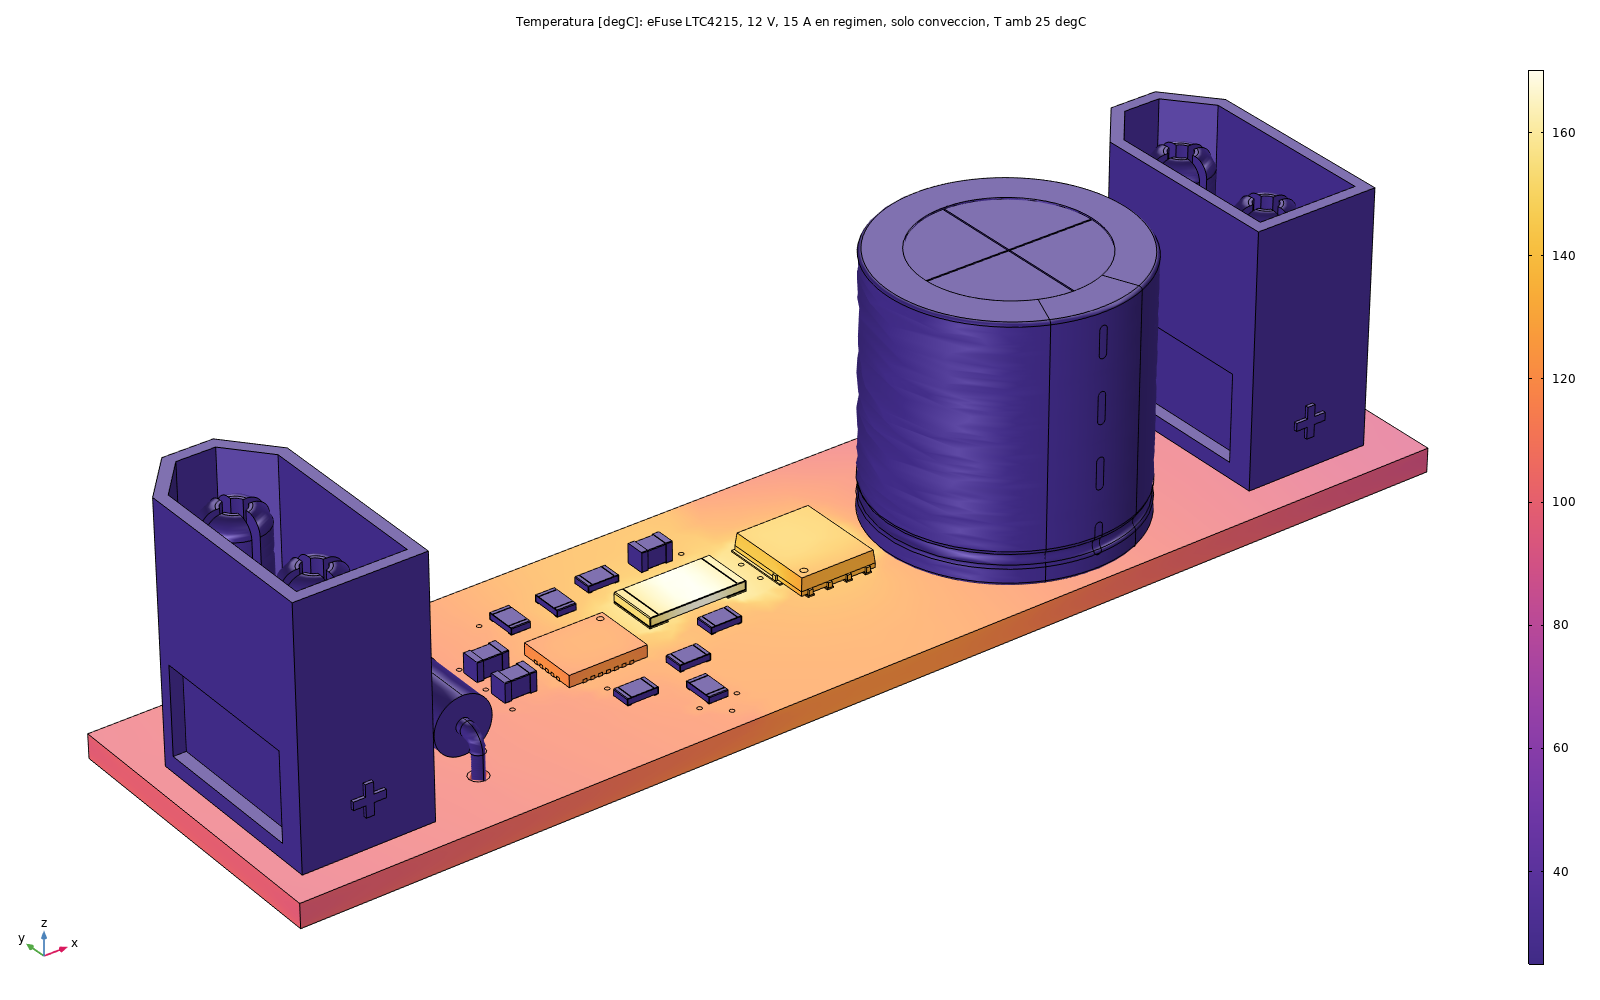
\includegraphics[width=0.85\linewidth]{figures/fem_15A_isometric.png}
\caption{Temperature at \SI{12}{\volt}, \SI{15}{\ampere}, convection only, copper heating and thermal vias
included. R5 (center) is the hottest part, followed by Q1 (right of R5); the whole power path is hot because
the pours themselves dissipate \SI{1.6}{\watt}.}
\end{figure}

\begin{figure}[H]
\centering
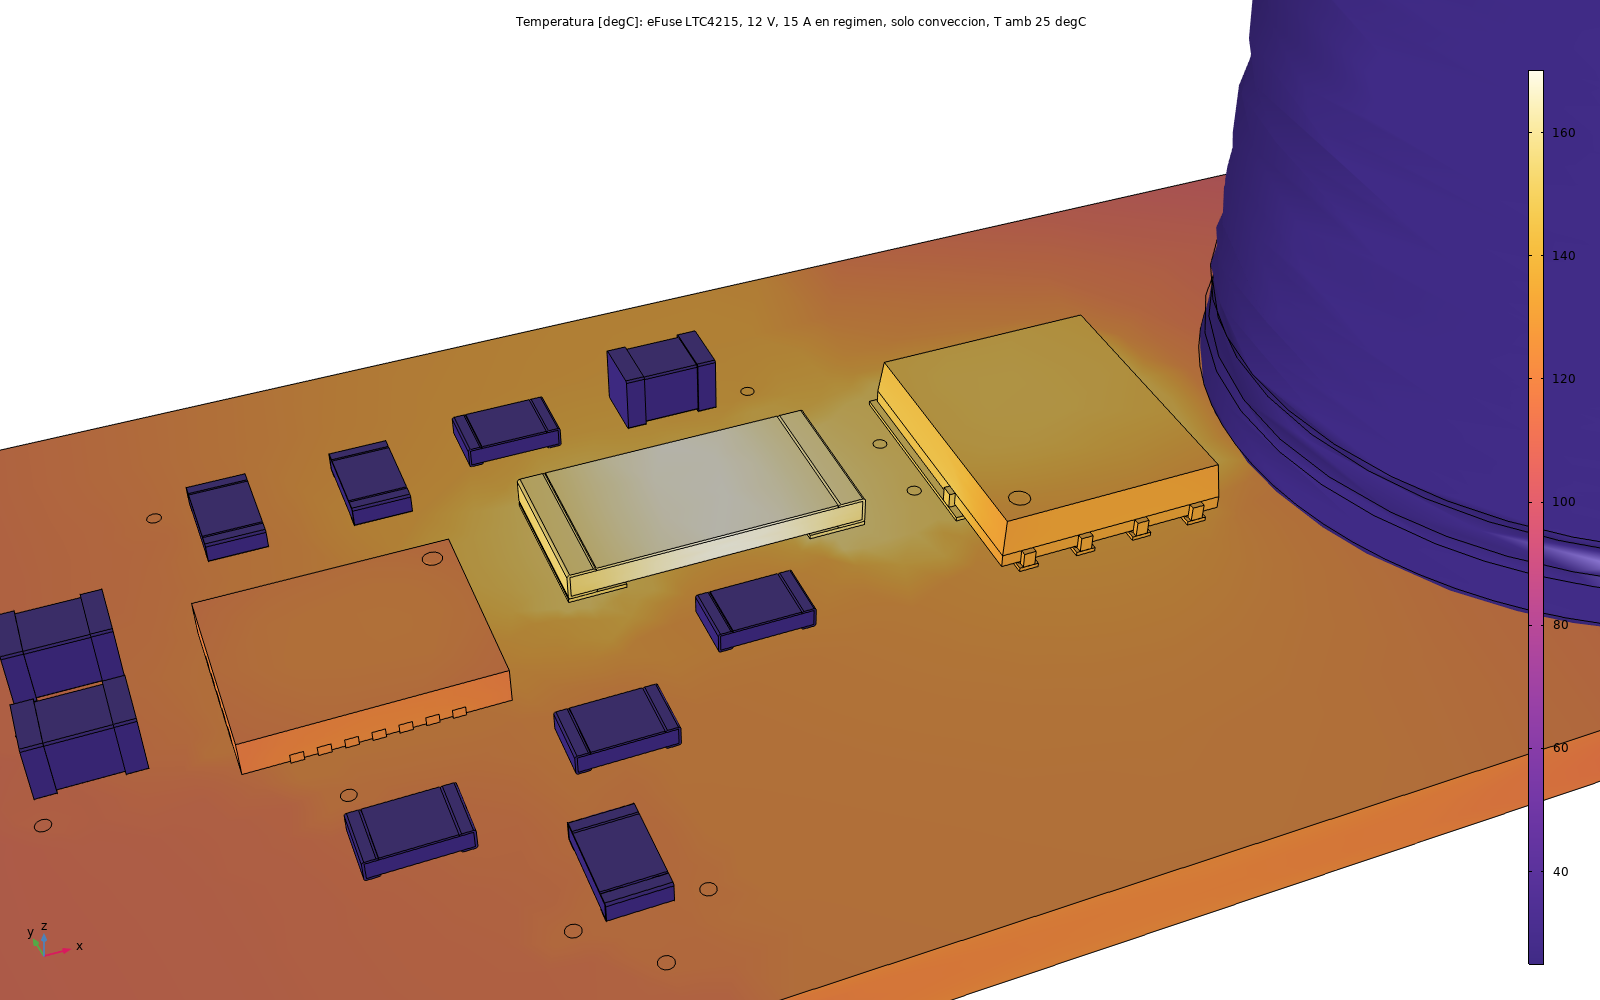
\includegraphics[width=0.85\linewidth]{figures/fem_15A_closeup_R5_Q1.png}
\caption{Close-up of R5 and Q1.}
\end{figure}

\begin{figure}[H]
\centering
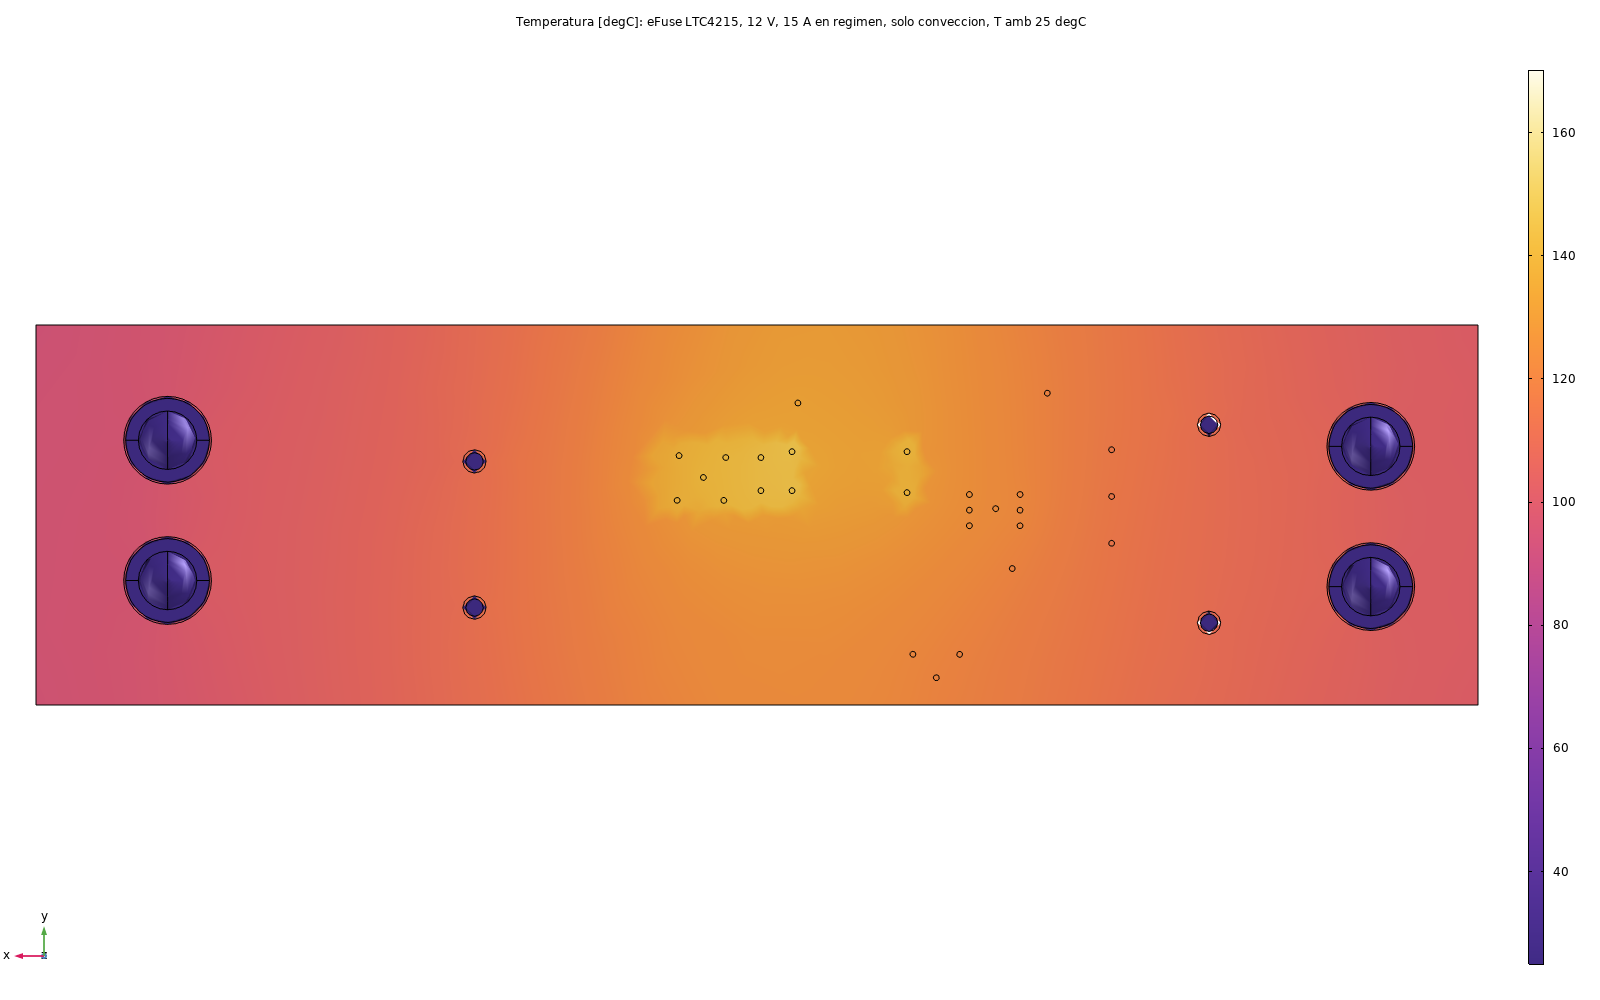
\includegraphics[width=0.85\linewidth]{figures/fem_15A_bottom.png}
\caption{Bottom side (seen from below, so mirrored left--right). The warmest spots are the new SENSE$-$
island with its vias under R5/Q1 and the two +12V vias: the vias carry heat to the bottom layer.}
\label{fig:fembottom}
\end{figure}

\paragraph{Current sweep (final board, convection only, $R_{DS(on)}$ at \SI{25}{\celsius}).}
$P$ is R5 + Q1 + U1 only; the copper adds roughly as much again.
\begin{center}
\begin{tabular}{@{}ccccc@{}}
\toprule
$I$ & $P$ (parts) & R5 max & Q1 junction & U1 max \\
\midrule
\SI{5}{\ampere} & \SI{0.22}{\watt} & \SI{45.7}{\celsius} & \SI{43.2}{\celsius} & \SI{41.8}{\celsius} \\
\SI{7.5}{\ampere} & \SI{0.45}{\watt} & \SI{66.1}{\celsius} & \SI{60.6}{\celsius} & \SI{56.1}{\celsius} \\
\SI{10}{\ampere} & \SI{0.78}{\watt} & \SI{93.5}{\celsius} & \SI{83.9}{\celsius} & \SI{74.8}{\celsius} \\
\SI{12.5}{\ampere} & \SI{1.19}{\watt} & \SI{127.9}{\celsius} & \SI{113.0}{\celsius} & \SI{98.2}{\celsius} \\
\SI{15}{\ampere} & \SI{1.70}{\watt} & \SI{170.2}{\celsius} & \SI{148.9}{\celsius} & \SI{126.8}{\celsius} \\
\bottomrule
\end{tabular}
\end{center}

\subsection{Findings}

\begin{itemize}
\item \textbf{The copper heating is the dominant missing piece}: \SI{1.6}{\watt}, adding
\SI{30}{}--\SI{40}{\celsius} to every part. The first pass, without it, was optimistic.
\item \textbf{The thermal vias work, but the gain is modest}: \SI{-9}{\celsius} on R5 and
\SI{-10}{\celsius} on Q1, in every variant. They help move heat to B.Cu, but the problem is now the total
heat on a small board, not only how it leaves R5 and Q1.
\item \textbf{Continuous \SI{15}{\ampere} is not thermally safe in still air.} With convection only, Q1's
junction sits right at its \SI{150}{\celsius} $T_{J,max}$ (\SI{164}{\celsius} with a hot $R_{DS(on)}$),
and R5 reaches \SI{170}{\celsius}, at or above typical 2512 maximum operating temperatures
(\SI{155}{}--\SI{170}{\celsius}). Counting radiation (realistic for a solder-masked board) it is
\SI{112}{}--\SI{124}{\celsius} on Q1 and \SI{133}{}--\SI{141}{\celsius} on R5: within limits but with
little margin.
\item \textbf{R5, not the MOSFET, is still the hottest component} -- same pattern as the LM2596 project,
where the catch diode, not the regulator IC, limited the design.
\item \textbf{\SI{12.5}{\ampere} continuous is comfortable}: \SI{128}{\celsius} on R5 and \SI{113}{\celsius}
on Q1 even with convection only.
\item \textbf{To reach \SI{15}{\ampere} continuous}, in order of effect: 2\,oz copper (halves the
\SI{1.6}{\watt} copper loss), wider/shorter power pours, a metal-strip R5 ($\geq$\SI{2}{\watt},
higher temperature rating), any airflow, and a +12V island on B.Cu so the two dangling vias work.
\end{itemize}

\paragraph{Not modeled.} The XT60 connectors and the large capacitor sit \SI{85}{\micro\meter} above the
board in the STEP with no solder under them, so they are thermally floating; in reality the connectors and
the input/output cables act as heat sinks (and as extra $I^2R$ sources at their contacts). Vias carry heat
but not current between layers in the electrical model.

% ======================================================================
\section{Known Limitations}

\begin{itemize}
\item \textbf{No reverse blocking.} As shown in Section~\ref{sec:results}, a single N-channel series
MOSFET's body diode will always pass current from output to input if the output is briefly higher than the
input, independent of the LTC4215's own gate control. Acceptable for this project's scope (inrush/OC
protection into a load), not acceptable where true input disconnection is required.
\item \textbf{Simulation-only substitute part.} The TVS (BZX84C15L in place of P6KE16A) is a
SPICE-availability substitute only -- the real BOM/PCB correctly specifies P6KE16A (Section~\ref{sec:tvs},
Section~\ref{sec:pcb}).
\item \textbf{No I$^2$C/ADC validation.} Monitoring, alerting, and the 8-bit ADC are real LTC4215 features
left entirely untested here (Section~\ref{sec:scope}).
\item \textbf{Thermal: continuous \SI{15}{\ampere} not safe in still air.} With the copper's own
\SI{1.6}{\watt} of $I^2R$ included, COMSOL gives \SI{170}{\celsius} on R5 and \SI{149}{\celsius} on Q1's
junction (convection only, with the thermal vias); \SI{12.5}{\ampere} continuous is comfortable
(Section~\ref{sec:thermal}).
\item \textbf{Silkscreen overlap.} DRC reports cosmetic silkscreen-clearance warnings around the densely
packed U1/divider area. Not addressed -- irrelevant with no physical build planned (Section~\ref{sec:pcb}).
\end{itemize}

% ======================================================================
\section{Pending}

\begin{pending}
\begin{itemize}
\item Physical build/measurement -- out of scope for this project (simulation + layout only, confirmed at
project start), unlike \texttt{RLC\_PID\_UNI}.
\item Follow-on STM32 + I$^2$C telemetry project (Section~\ref{sec:scope}).
\item For continuous \SI{15}{\ampere}: 2\,oz copper and/or wider pours, a specific metal-strip R5, and a
+12V island on B.Cu for the two dangling vias -- then re-run the FEM (the script regenerates everything
from the \texttt{.kicad\_pcb}).
\end{itemize}
\end{pending}

% ======================================================================
\section{Conclusions}

A 12\,V hot-swap/eFuse front-end built around the LTC4215 was designed from the manufacturer's own
reference circuit, with every UV/OV/FB threshold independently re-derived and numerically cross-checked
against the datasheet's comparator thresholds rather than copied blindly. LTspice simulation confirmed all
three headline behaviors of the design: a soft-start-controlled inrush whose peak current lands on the
calculated \SI{5}{\ampere} circuit-breaker target, fully automatic recovery from an undervoltage event
(with a real, non-obvious $\approx\SI{100}{\milli\second}$ restart delay), and a permanent, non-resettable
latch-off on a hard output short. Two simulation pitfalls specific to this IC's behavior (a flat-DC source
hiding the power-up transient, and the internal \SI{100}{\milli\second} startup-sequencer delay) are
documented in Section~\ref{sec:pitfalls} so they are not re-discovered from scratch on a future project
using the same IC family.

The KiCad schematic and 2-layer PCB layout carry the design through to a fabricable, ERC/DRC-clean board:
a real, independently-verified QFN-24 part (not blindly trusted from its distributor library), a corrected
MOSFET footprint/symbol pin mapping, a Kelvin-connected sense resistor, and dedicated copper pours sized
for the \SI{15}{\ampere} steady-state current. Two more IC/package-specific gotchas (fine-pitch QFN copper
clearance and solder-mask aperture bridging, Section~\ref{sec:pcb}) are documented alongside the two
simulation pitfalls, for the same reason.

A COMSOL steady-state model at the continuous \SI{12}{\volt}/\SI{15}{\ampere} point, with the current
flow in the copper solved together with the heat (Section~\ref{sec:thermal}), found that \textbf{the pours
themselves dissipate \SI{1.6}{\watt}}, as much as all the components together, and that the \textbf{sense
resistor R5}, not the MOSFET, is the hottest part. Thermal vias under R5 and Q1, added in response to the
first pass, lower both by about \SI{10}{\celsius}, but in still air continuous \SI{15}{\ampere} still puts
R5 at \SI{170}{\celsius} and Q1's junction at its \SI{150}{\celsius} limit; \SI{12.5}{\ampere} continuous
is comfortable, and \SI{15}{\ampere} needs heavier copper, a metal-strip R5 or airflow.

\end{document}
